\documentclass[11pt,a4paper]{article}
\usepackage[margin=24mm,headheight=15pt]{geometry}
\usepackage[T1]{fontenc}
\usepackage{lmodern,microtype,amsmath,amssymb,booktabs,tabularx,array,graphicx,xcolor,fancyhdr,listings,enumitem}
\usepackage[colorlinks=true,linkcolor=black,urlcolor=blue,citecolor=black]{hyperref}
\hypersetup{pdftitle={Rainfall Prediction Across Three Indian Cities Using Multilinear Regression},pdfauthor={Yug Bhushan}}
\definecolor{ink}{HTML}{234D6B}
\setlength{\parskip}{6pt}
\setlength{\parindent}{0pt}
\setlist{nosep,leftmargin=1.5em}
\renewcommand{\arraystretch}{1.2}
\pagestyle{fancy}\fancyhf{}\fancyhead[L]{\small Rainfall Prediction Using Multiple Linear Regression}\fancyhead[R]{\small Yug Bhushan}\fancyfoot[C]{\thepage}
\lstset{language=Python,basicstyle=\ttfamily\scriptsize,breaklines=true,columns=fullflexible,keepspaces=true,showstringspaces=false,frame=single,rulecolor=\color{black!20},numbers=left,numberstyle=\tiny\color{black!50},numbersep=7pt,xleftmargin=10pt,framexleftmargin=5pt,aboveskip=8pt,belowskip=8pt}
\newcommand{\R}{\mathbb{R}}
\newcommand{\sectionpage}[1]{\clearpage\section{#1}}
\begin{document}
\begin{titlepage}
\centering
\vspace*{22mm}
{\Large\scshape Term Paper\par}
\vspace{16mm}
{\huge\bfseries Rainfall Prediction Across Three Indian Cities Using Multilinear Regression\par}
\vspace{9mm}
{\large Matrix Least Squares, Python Implementation,\\and Statistical Validation\par}
\vspace{24mm}
{\Large Yug Bhushan\par}
\vspace{3mm}
{\large 2025CH71601\par}
\vspace{7mm}
Department of Chemical Engineering\\
Indian Institute of Technology Delhi
\vfill
{\large Project period: November 2025\par}
\vspace{12mm}
\end{titlepage}

\section*{Abstract}
\addcontentsline{toc}{section}{Abstract}
Rainfall prediction links meteorological observations with decisions in water management, agriculture, drainage, and industrial operations. This paper develops the mathematical and computational framework for a multiple linear regression model for Delhi, Chennai, and Agra. Temperature, relative humidity, wind speed, surface pressure, and rainfall history form the predictor set. The regression coefficients are obtained through matrix least squares, and predictive performance is examined using Pearson correlation, mean squared error, root mean squared error, mean absolute error, and the coefficient of determination.

A central concern is the definition of prediction time. A model that estimates rainfall using weather observed during the same day is different from a model that forecasts the following day. A one-day-ahead formulation is therefore specified for the reproducible implementation in this paper. The workflow preserves calendar dates, separates earlier training observations from later test observations, and compares regression with persistence and training-mean baselines. The least-squares equations are derived, numerical conditioning is discussed, and a worked example demonstrates why high correlation alone cannot establish forecast accuracy.

The supplied project summary reports a correlation range of $R=0.95$--$0.99$ across the three cities. Raw observations, fitted coefficients, and city-specific validation outputs were not supplied. This range is consequently retained as a reported project outcome, rather than presented as an independently reproduced test result. Numerical examples are explicitly illustrative. The paper provides a complete methodological account and executable Python appendix; the original dataset remains necessary to establish the empirical performance of the three city models.

\textbf{Keywords:} rainfall prediction; multiple linear regression; ordinary least squares; meteorological data; chronological validation; Python.

\vspace{5mm}
\subsection*{Scope of this manuscript}
The model family, three cities, meteorological variables, Python least-squares implementation, and reported correlation range follow the supplied project description. The forecast horizon, chronological split, data checks, and baseline comparisons are specified here as a reproducible validation protocol. They should not be read as undocumented details of the original experiment. No station, observation period, sample count, fitted coefficient, or city-wise MSE has been invented.

\clearpage
\tableofcontents

\clearpage
\section*{Nomenclature}
\addcontentsline{toc}{section}{Nomenclature}
\begin{tabularx}{\textwidth}{@{}lXl@{}}\toprule
Symbol & Meaning & Unit \\\midrule
$c$ & City index: Delhi, Chennai, or Agra & --\\
$t$ & Daily forecast-origin index & day\\
$Y_{c,t}$ & Observed daily rainfall accumulation & mm\\
$\widehat Y_{c,t+1}$ & Predicted rainfall for the next daily interval & mm\\
$T_{c,t}$ & Daily air temperature predictor & $^\circ$C\\
$H_{c,t}$ & Relative humidity predictor & \%\\
$W_{c,t}$ & Wind-speed predictor & m s$^{-1}$\\
$P_{c,t}$ & Surface-pressure predictor & hPa\\
$n$ & Number of usable supervised observations & --\\
$p$ & Number of predictors, excluding the intercept & --\\
$X$ & Design matrix, including an intercept column & mixed\\
$\boldsymbol\beta$ & Vector of regression coefficients & mixed\\
$\boldsymbol\varepsilon$ & Unexplained component of rainfall & mm\\
$e_i$ & Residual, $y_i-\widehat y_i$ & mm\\
$R$ & Pearson correlation of observations and predictions & --\\
$R^2$ & Coefficient of determination & --\\
SSE & Sum of squared prediction errors & mm$^2$\\
MSE & Mean squared prediction error & mm$^2$\\
RMSE & Root mean squared prediction error & mm\\
MAE & Mean absolute prediction error & mm\\
$\mu_j,s_j$ & Training-set mean and standard deviation of feature $j$ & feature unit\\
$\kappa(X)$ & Condition number of the design matrix & --\\
\bottomrule\end{tabularx}

\subsection*{Terminology}
The project uses the term \emph{multilinear regression}. Here it means \emph{multiple linear regression}: the response is linear in the unknown coefficients and depends additively on several predictors. It does not imply that interactions between all predictor variables are included. A polynomial or interaction model may still be linear in its coefficients, but it is an extension of the additive baseline examined here.

Daily rainfall is an accumulation over a defined interval. The date convention, time zone, and measurement window must be consistent across predictors and target. A daily average predictor is considered available only after its averaging interval has ended.

\sectionpage{Introduction}
\subsection{Motivation and engineering relevance}
Rainfall is an important input to water balances. In a storage system, the incoming rainfall volume depends on rainfall depth, contributing area, and the fraction that becomes runoff. For a simple catchment representation,
\begin{equation}
V_{\mathrm{runoff}}\approx C A Y/1000,
\end{equation}
where $A$ is area in m$^2$, $Y$ is rainfall depth in mm, and $C$ is a dimensionless runoff coefficient. The resulting volume is in m$^3$. This approximation illustrates the practical consequence of rainfall error: a bias in predicted rainfall propagates into expected inflow. It does not replace a hydrological routing model.

For chemical engineering facilities, rainfall can affect stormwater storage, outdoor material handling, wastewater dilution, and the scheduling of water-intensive operations. A statistical rainfall model offers a useful exercise in relating measured environmental variables to a response, checking assumptions, and evaluating whether a model improves a decision-relevant baseline.

\subsection{Why use a linear model?}
A linear regression model is inexpensive to fit and easy to inspect. Its coefficients reveal the fitted change in rainfall associated with a predictor when the other included predictors are held fixed. This makes it a useful baseline before adopting a more flexible model. The mathematical foundation also provides a direct connection between optimization, linear algebra, and uncertainty.

Rainfall nevertheless presents difficulties. Many days can have zero rainfall, while a few events account for large accumulations. Temperature, humidity, pressure, and wind may interact, and a local daily record cannot fully represent atmospheric circulation or storm movement. An additive linear model is therefore an approximation to the conditional mean, rather than a physical law of precipitation.

\subsection{Objectives}
This paper aims to:
\begin{enumerate}
\item formulate rainfall prediction for Delhi, Chennai, and Agra using a consistent predictor set;
\item derive the ordinary least-squares estimator and explain a stable numerical solution;
\item describe data cleaning, temporal alignment, and leakage-resistant validation;
\item distinguish correlation from error magnitude and baseline-relative skill;
\item interpret the supplied project result at the level supported by the evidence; and
\item provide executable Python code for reproducing the analysis when observations are available.
\end{enumerate}

\subsection{Organization}
Section 2 defines the observations and prediction target. Sections 3 and 4 develop the mathematics and computational workflow. Sections 5 and 6 explain validation and present a worked numerical example. Sections 7 and 8 discuss the reported project outcome, limitations, and conclusions. Appendix A contains the implementation, and Appendix B documents its use.

\sectionpage{Study Design and Data Requirements}
\subsection{Three-city comparison}
Delhi, Chennai, and Agra are the locations named in the supplied project description. Separate city models are used in the implementation so that every location has its own intercept, slopes, and validation errors. This avoids imposing a common response to weather across all three locations.

Seasonal differences also matter. For example, the India Meteorological Department identifies October--December as the northeast monsoon season and an important rainy season for Tamil Nadu and Puducherry \cite{imd}. This regional context motivates checking seasonal performance in Chennai. The present manuscript does not assign a station climatology or monthly rainfall total to any city without the corresponding observations.

\subsection{Required observation schema}
\begin{table}[h!]\centering\small
\begin{tabularx}{\textwidth}{@{}lXl@{}}\toprule
CSV column & Definition & Required unit\\\midrule
\texttt{date} & Date of the completed daily observation interval & YYYY-MM-DD\\
\texttt{city} & Exactly Delhi, Chennai, or Agra & text\\
\texttt{temperature} & Daily temperature summary, consistently defined & $^\circ$C\\
\texttt{humidity} & Daily relative humidity summary & \%\\
\texttt{wind\_speed} & Daily wind-speed summary at a documented height & m s$^{-1}$\\
\texttt{pressure} & Daily surface pressure & hPa\\
\texttt{rainfall} & Daily accumulated rainfall & mm\\\bottomrule
\end{tabularx}
\caption{Input contract for the reproducible daily implementation.}
\end{table}
For an empirical study, this schema must be accompanied by the provider, station identifier or grid coordinates, observation dates, missing-value codes, and measurement conventions. Surface pressure and sea-level pressure are different quantities and should not be mixed. Pressure in kPa must be multiplied by ten before entering a model specified in hPa.

\subsection{Observation sources and provenance}
An official station record or a documented meteorological data product can support this analysis. NASA POWER is one possible source for a future reconstruction: its Daily API supports daily data requests and several output formats \cite{nasa}. It is not identified here as the source of the original project because that information was not supplied. Gridded estimates should also be described as gridded estimates rather than as measurements taken at a city weather station.

\subsection{Target and forecast origin}
The reproducible formulation forecasts $Y_{c,t+1}$ after day $t$ has ended, using the completed daily predictors $T_{c,t},H_{c,t},W_{c,t},P_{c,t},Y_{c,t}$. Rainfall on day $t$ is a lagged predictor relative to the target. If the original work instead estimated $Y_{c,t}$ from weather observed during day $t$, it should be described as contemporaneous rainfall estimation. Using the response itself as an input would create target leakage.

\sectionpage{Mathematical Theory and Least-Squares Derivation}
\subsection{Regression equation}
For each city, the proposed one-day-ahead additive model is
\begin{equation}\label{eq:model}
Y_{c,t+1}=\beta_{0,c}+\beta_{T,c}T_{c,t}+\beta_{H,c}H_{c,t}
+\beta_{W,c}W_{c,t}+\beta_{P,c}P_{c,t}+\beta_{L,c}Y_{c,t}+\varepsilon_{c,t+1}.
\end{equation}
The error term represents omitted influences, measurement uncertainty, and departures from the chosen functional form. There are five predictors and six fitted coefficients. The model is fitted independently for each city; the city subscript is suppressed below for readability.

For $n$ usable predictor--target pairs, write
\begin{equation}
\mathbf y=X\boldsymbol\beta+\boldsymbol\varepsilon,\qquad
X=\begin{bmatrix}
1&T_1&H_1&W_1&P_1&Y_1\\
1&T_2&H_2&W_2&P_2&Y_2\\
\vdots&\vdots&\vdots&\vdots&\vdots&\vdots\\
1&T_n&H_n&W_n&P_n&Y_n
\end{bmatrix}.
\end{equation}
Each response in $\mathbf y$ belongs to the day after the predictor row. Thus $X\in\R^{n\times6}$, $\boldsymbol\beta\in\R^6$, and $\mathbf y\in\R^n$.

\subsection{Minimization of squared residuals}
Ordinary least squares minimizes
\begin{align}
S(\boldsymbol\beta)&=(\mathbf y-X\boldsymbol\beta)^T(\mathbf y-X\boldsymbol\beta)\\
&=\mathbf y^T\mathbf y-2\boldsymbol\beta^TX^T\mathbf y+
\boldsymbol\beta^TX^TX\boldsymbol\beta.
\end{align}
Differentiating with respect to the coefficient vector gives
\begin{equation}
\nabla S=-2X^T\mathbf y+2X^TX\boldsymbol\beta.
\end{equation}
At a minimum, the gradient vanishes, leading to the normal equations:
\begin{equation}\label{eq:normal}
X^TX\widehat{\boldsymbol\beta}=X^T\mathbf y.
\end{equation}
If $X$ has full column rank, $X^TX$ is positive definite and the unique solution is
\begin{equation}\label{eq:inverse}
\widehat{\boldsymbol\beta}=(X^TX)^{-1}X^T\mathbf y.
\end{equation}
Equation \eqref{eq:inverse} is an analytical expression, not a recommendation to form an explicit inverse in code. Because the objective is convex, a full-rank stationary point is the global minimum.

\subsection{Projection interpretation}
The fitted response $\widehat{\mathbf y}=X\widehat{\boldsymbol\beta}$ lies in the column space of $X$. The residual vector obeys $X^T\mathbf e=\mathbf0$, meaning that it is orthogonal to each design column on the training data. With an intercept, training residuals sum to zero. These identities do not guarantee zero bias on unseen observations.

\clearpage
\subsection{Numerical conditioning and stable solution}
Weather variables have different magnitudes and may be strongly associated with one another. Pressure values near a large reference level, for example, can make the intercept and pressure column poorly scaled. In the 2-norm, forming normal equations squares the condition number for a full-rank design:
\begin{equation}
\kappa_2(X^TX)=\kappa_2(X)^2.
\end{equation}
Consequently, a small numerical perturbation can be amplified. A direct least-squares routine avoids explicitly computing $(X^TX)^{-1}$. The implementation uses \texttt{numpy.linalg.lstsq}, which returns the least-squares coefficients together with rank and singular values \cite{numpy}.

For insight, a thin QR factorization $X=QR$ transforms the minimization into
\begin{equation}
R\widehat{\boldsymbol\beta}=Q^T\mathbf y,
\end{equation}
provided $X$ has full column rank. A singular value decomposition $X=U\Sigma V^T$ gives the pseudoinverse representation
\begin{equation}
\widehat{\boldsymbol\beta}=V\Sigma^+U^T\mathbf y.
\end{equation}
Very small singular values indicate directions of weak identification. A model may predict reasonably while individual slopes remain unstable. The code rejects a rank-deficient design rather than silently treating its coefficients as uniquely identified.

\subsection{Standardization and original-unit coefficients}
Using training statistics only, each feature is transformed as
\begin{equation}
z_{ij}=(x_{ij}-\mu_j)/s_j.
\end{equation}
If the standardized fitted model is $\widehat y=a+\sum_jb_jz_j$, then
\begin{equation}
\beta_j=b_j/s_j,\qquad
\beta_0=a-\sum_j b_j\mu_j/s_j.
\end{equation}
These equations convert the model back to its physical units. Standardization improves scale balance but does not remove multicollinearity. A constant predictor has $s_j=0$ and must be removed or otherwise treated; the appendix raises an error in that case.

\subsection{Assumptions and interpretation}
The conditional mean is approximated by the chosen linear form. Exogeneity, expressed as $E[\varepsilon\mid X]=0$, is required for the usual conditional unbiasedness interpretation. Constant error variance and independent errors are additional assumptions for classical standard-error formulas. Normal errors are not required to calculate least-squares coefficients, but they enter exact small-sample parametric inference.

Daily rainfall errors may be heteroscedastic and serially correlated. The basic point predictions remain computable, but textbook confidence intervals can be misleading. This paper therefore emphasizes chronological prediction errors rather than unverified significance tests. Estimated slopes describe conditional associations; they do not establish causal effects of weather interventions.

\sectionpage{Data Processing and Computational Methodology}
\subsection{Calendar alignment and quality control}
The processing sequence begins with parsing dates, separating cities, checking duplicate city--date records, and sorting each city chronologically. Every city is reindexed to a complete daily calendar before the following day's rainfall is created. This step is essential: shifting after dropping missing dates could accidentally pair Monday's predictors with Wednesday's rainfall.

The code treats nonnumeric and nonfinite values as missing. Negative rainfall, negative wind speed, humidity outside 0--100\%, and nonpositive pressure invalidate a predictor row. Known provider-specific missing codes must be converted before running the script. A negative temperature is not automatically an error. A zero rainfall value is a valid dry-day observation and must not be discarded.

The baseline implementation uses complete cases after calendar alignment. Missing rainfall is never replaced by zero. This choice is transparent, although it can reduce the sample and bias evaluation if storm periods are disproportionately missing. More advanced imputation must be fitted on training data and must respect which observations were available at forecast time.

\subsection{Training and test design}
The proposed split assigns the earliest approximately 70\% of usable daily pairs to training and the latest approximately 30\% to testing. An additional conservative boundary purge excludes training rows whose target date reaches the first test forecast-origin date. This preserves temporal ordering at the split. The exact retained counts depend on calendar gaps and should be reported from the run output.

The split ratio is a protocol choice, not a recovered fact about the original project. A useful test window should cover the relevant rainy and dry seasons. If a short record leaves only one season in the holdout, the resulting score should be interpreted for that season. Expanding-window validation is an appropriate extension when enough years are available; time-ordered splitting is supported by established validation tools \cite{timesplit}.

\subsection{Model fitting and repeated forecast issue times}
Training means and standard deviations are calculated once. The standardized training design is solved by least squares, and the resulting coefficients are held fixed during testing. Each test prediction uses the meteorological observations from its own completed origin day. This is a sequence of one-day-ahead forecasts; it is not a single forecast of the entire test interval issued at the end of training.

Any feature selection, clipping choice, transformation, or hyperparameter tuning should use training or validation periods. The final test period is reserved for assessment. Learning preprocessing quantities from the full dataset would leak test information into fitting \cite{pitfalls}.

\subsection{Outputs and traceability}
The appendix writes model and baseline metrics, original-unit coefficients, dated observations and predictions, residuals, and diagnostic figures. These outputs provide a direct trail from input rows to reported performance. The script performs a single chronological holdout; it does not claim to implement expanding-window cross-validation, seasonal scoring, or calibrated prediction intervals.

\sectionpage{Statistical Validation and Diagnostic Analysis}
Let $m$ denote the number of test observations and let $e_i=y_i-\widehat y_i$. All compared models must be evaluated on the same dated target rows.

\subsection{Error magnitude}
\begin{align}
\mathrm{MSE}&=\frac{1}{m}\sum_{i=1}^m e_i^2,&
\mathrm{RMSE}&=\sqrt{\mathrm{MSE}},\\
\mathrm{MAE}&=\frac{1}{m}\sum_{i=1}^m|e_i|,&
\mathrm{Bias}&=\frac{1}{m}\sum_{i=1}^m(\widehat y_i-y_i).
\end{align}
MSE penalizes large errors strongly and has units of mm$^2$. RMSE and MAE retain the rainfall unit, mm. Positive bias indicates average overprediction. These measures describe different aspects of performance and should be reported together \cite{metrics}.

\subsection{Correlation and coefficient of determination}
Pearson correlation is
\begin{equation}
R=\frac{\sum_i(y_i-\bar y)(\widehat y_i-\overline{\widehat y})}
{\sqrt{\sum_i(y_i-\bar y)^2\sum_i(\widehat y_i-\overline{\widehat y})^2}}.
\end{equation}
It describes linear association and is undefined if either series has zero variance. By contrast,
\begin{equation}
R^2=1-\frac{\sum_i(y_i-\widehat y_i)^2}{\sum_i(y_i-\bar y)^2}
\end{equation}
compares squared error with the constant test-sample mean reference. Test $R^2$ can be negative. Squaring Pearson $R$ does not generally yield predictive test $R^2$; equality has special conditions, such as an in-sample ordinary least-squares fit with an intercept and a nonconstant response. Correlation is also not a percentage accuracy measure.

\subsection{Baselines and skill}
A persistence forecast sets $\widehat Y_{t+1}=Y_t$. A second baseline predicts the training-period mean rainfall. These are deployable references because their required information is available at forecast time. MSE skill relative to a chosen baseline is
\begin{equation}
\mathrm{Skill}=1-\frac{\mathrm{MSE}_{\mathrm{model}}}{\mathrm{MSE}_{\mathrm{baseline}}},
\end{equation}
when the denominator is positive. Positive skill indicates improvement. A seasonal climatology fitted only to training years is a useful further comparator but is not implemented in the appendix.

\subsection{Residual and event-level checks}
An observed-versus-predicted plot should be compared with the identity line. Residuals against time reveal runs of underprediction; residuals against fitted values can expose changing variance. Seasonal subsets and large-event errors should be inspected separately because a good all-day score can conceal poor heavy-rainfall performance. Thresholds for event analysis must be declared in advance or based on training data. Negative raw OLS predictions should be counted; clipping them at zero creates a distinct postprocessed model whose metrics require separate reporting.

\sectionpage{Worked Numerical Example}
\subsection{Purpose and illustrative observations}
The six pairs below are constructed solely to demonstrate the evaluation formulas. They are not observations from Delhi, Chennai, or Agra, and they do not reproduce the supplied correlation range.

\begin{table}[h!]\centering
\begin{tabular}{@{}rrrrr@{}}\toprule
Index & Observed (mm) & Predicted (mm) & Residual (mm) & Squared error (mm$^2$)\\\midrule
1&0&1&$-1$&1\\2&2&3&$-1$&1\\3&5&4&1&1\\4&10&12&$-2$&4\\5&20&18&2&4\\6&35&32&3&9\\\bottomrule
\end{tabular}
\caption{Illustrative test pairs used only for arithmetic demonstration.}
\end{table}
The observed mean is 12 mm, SSE is 20 mm$^2$, and the total squared deviation from the observed mean is 890 mm$^2$. Therefore,
\begin{align*}
\mathrm{MSE}&=20/6=3.3333\ \mathrm{mm}^2,\\
\mathrm{RMSE}&=1.8257\ \mathrm{mm},\qquad \mathrm{MAE}=1.6667\ \mathrm{mm},\\
\mathrm{Bias}&=-0.3333\ \mathrm{mm},\\
R^2&=1-20/890=0.97753,\qquad R=0.99487.
\end{align*}
The largest observation is underpredicted by 3 mm even though the correlation is very high. This is why individual event errors remain informative.

\begin{figure}[h!]\centering
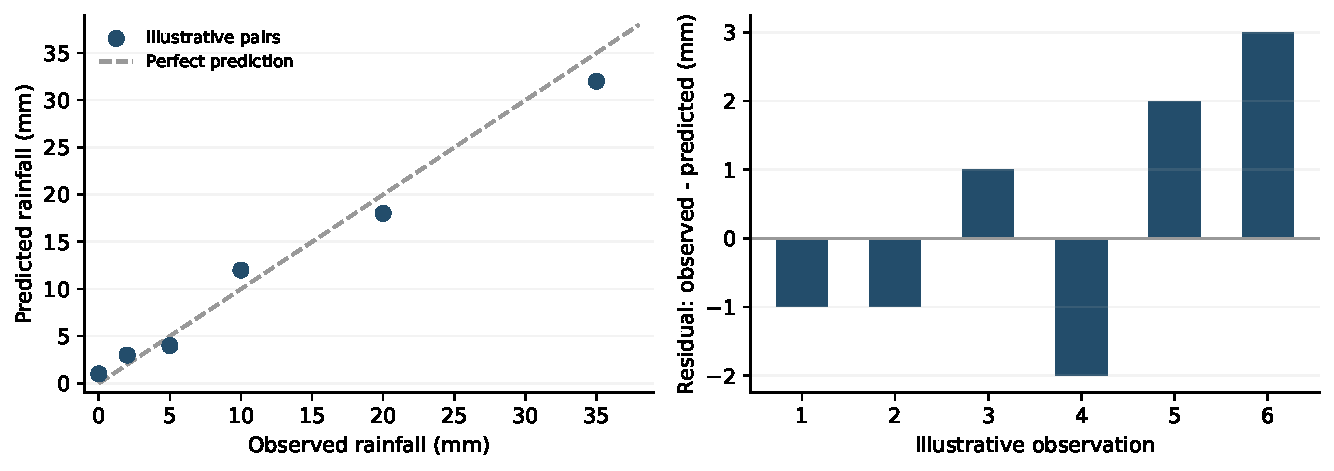
\includegraphics[width=\textwidth]{worked_example.pdf}
\caption{Illustrative observations and residuals from Table 2. These graphics are not city model results.}
\end{figure}

\clearpage
\subsection{High correlation with systematic error}
Consider a second illustrative predictor, $\widehat y_i=y_i+10$ mm, on the same six observations. Every prediction is too high by 10 mm, yet Pearson correlation is exactly one. The error measures are
\begin{equation}
\mathrm{MSE}=100\ \mathrm{mm}^2,\quad \mathrm{RMSE}=10\ \mathrm{mm},\quad
R^2=1-600/890=0.32584.
\end{equation}
The example isolates calibration error: correlation measures the alignment of fluctuations but is unchanged by a constant offset. A claim of $R=0.99$ is thus insufficient without error magnitudes, bias, test dates, and a baseline.

\subsection{An illustrative prediction calculation}
To demonstrate coefficient interpretation, suppose a model has the following deliberately chosen equation:
\begin{equation}\begin{split}
\widehat Y_{t+1}={}&2+0.15(T_t-25)+0.10(H_t-60)\\
&+0.40W_t-0.05(P_t-1000)+0.30Y_t.
\end{split}\end{equation}
For $T_t=30\ ^\circ$C, $H_t=80\%$, $W_t=2$ m s$^{-1}$, $P_t=996$ hPa, and $Y_t=5$ mm,
\begin{equation}
\widehat Y_{t+1}=2+0.75+2+0.8+0.2+1.5=7.25\ \mathrm{mm}.
\end{equation}
These coefficients are illustrative and were not fitted to the project data. The centering constants change the intercept's interpretation, not the additive model family.

At fixed values of the remaining predictors, this example associates a ten percentage-point increase in humidity with a 1 mm increase in predicted rainfall. It associates a 2 hPa pressure increase with a 0.1 mm reduction. Neither statement is a universal weather relationship or a causal conclusion. The physical credibility and stability of fitted slopes would need checking against the actual city data.

\subsection{Propagation into an engineering estimate}
For a hypothetical catchment of $A=10{,}000$ m$^2$ and runoff coefficient $C=0.8$, a 3 mm rainfall error gives an approximate runoff-volume error of
\begin{equation}
|\Delta V|\approx C A|\Delta Y|/1000=24\ \mathrm{m}^3.
\end{equation}
This calculation is an application example, not a drainage design recommendation. It shows why an error stated in physical units can be more useful for engineering interpretation than a correlation coefficient alone.

\sectionpage{Reported Project Outcome and Discussion}
\subsection{Evidence available for this paper}
The supplied project summary states that a rainfall forecasting model was built from meteorological variables and that matrix least squares was implemented in Python. It identifies Delhi, Chennai, and Agra and reports $R=0.95$--$0.99$ across the three cities, with MSE and correlation used in validation. It does not provide the underlying files needed to recompute those measures.

\begin{table}[h!]\centering\small
\begin{tabularx}{\textwidth}{@{}lX@{}}\toprule
Item & Supported statement or current limitation\\\midrule
Model family & Multiple linear regression with matrix least squares, as reported in the supplied summary.\\
Locations & Delhi, Chennai, and Agra.\\
Reported correlation & $R=0.95$--$0.99$ across the cities; the mapping of values to individual cities is not supplied.\\
City-specific MSE & Not supplied; no numerical values are assigned in this paper.\\
Forecast lead time & Not specified in the summary; this paper proposes one-day-ahead prediction for reproducibility.\\
Observation record & Provider, station or grid, dates, frequency, and sample counts are not supplied.\\
Validation partition & Training/test dates and whether the stated range is in-sample or held-out are not supplied.\\
Fitted equations & Coefficients are not supplied; the equation in Section 6 is illustrative.\\\bottomrule
\end{tabularx}
\caption{Evidence status of the empirical claims.}
\end{table}

\subsection{Interpretation of the reported correlation range}
The stated range indicates strong positive linear association if it refers to observed and predicted rainfall on matched observations. It does not establish the size of forecast error, whether rainy days were selected, whether observations were aggregated, or whether a future period was held out. A defensible account should name the two series being correlated and identify the evaluation period.

High correlation in a seasonal aggregate may reflect a common annual cycle. A random split of adjacent daily observations may benefit from temporal dependence. Inclusion of target-day rainfall or weather that was unavailable at issue time can also create an overly optimistic forecasting claim. These are checks to perform on the original analysis, not conclusions that any of these errors occurred.

\subsection{What a completed city comparison should establish}
For each city, the empirical output should report source and location metadata; training and test dates; retained row counts; the fitted coefficients; $R$, $R^2$, MSE, RMSE, MAE, and bias; and the same metrics for baselines. It should also include a dated prediction file and residual diagnostics. The appendix produces the numerical outputs once a validated daily CSV is supplied. Until then, no ranking of Delhi, Chennai, and Agra by forecast accuracy is justified.

\sectionpage{Limitations, Extensions, and Conclusions}
\subsection{Model and data limitations}
The linear model imposes additivity and constant slopes across the fitted period. It can produce negative rainfall and may smooth extreme events. Unmeasured circulation, cloud development, and storm movement can limit the information available in local daily predictors. A lagged rainfall term captures some persistence but does not represent all weather dynamics.

Independent city fits are interpretable, although they do not share information between locations. Pooling the observations without city indicators would confound location differences with weather effects. A pooled extension should include location effects and, if supported by training validation, interactions between location and meteorological predictors.

Missingness, sensor changes, and nonstationarity can affect both fitted coefficients and evaluation. A longer record is valuable only if its measurement definitions remain consistent or documented adjustments are made. An operational system would require monitoring as new observations arrive.

\subsection{Potential improvements}
Ridge regression can stabilize coefficients when predictors are highly correlated. Seasonal sine and cosine terms can represent an annual cycle without introducing a discontinuity between December and January. Interaction terms can test whether the humidity association changes with temperature, provided their selection occurs within training validation.

A two-part model can separately estimate the probability of a wet day and the amount conditional on rain. Transforming rainfall with $\log(1+Y)$ is another possibility, but back-transformation requires care: exponentiating a predicted log mean does not generally recover the arithmetic mean rainfall. More flexible models should be compared on the same held-out targets, rather than assumed superior from complexity alone.

Forecast uncertainty is also relevant. Prediction intervals should be evaluated for empirical coverage on future periods. Temporal dependence means that an ordinary independent-row bootstrap or unadjusted textbook interval may be inappropriate; a justified temporal resampling or calibration strategy is needed.

\subsection{Conclusions}
Multiple linear regression provides an interpretable framework for relating rainfall to meteorological observations. Matrix least squares supplies the coefficient estimates, while rank checks, training-only standardization, and direct least-squares computation improve numerical reliability. A forecasting interpretation additionally requires a precise target interval and an explicit account of which predictors are available when a prediction is issued.

The supplied project summary reports $R=0.95$--$0.99$ across Delhi, Chennai, and Agra. This paper preserves that result as reported, without inventing city-specific errors or fitted equations. The worked calculations demonstrate that high correlation can coexist with systematic bias and substantial rainfall error. Empirical validation therefore requires chronological holdouts, physical-unit error metrics, baseline comparisons, and residual analysis. The accompanying implementation makes those checks reproducible once the original observations are available.

\appendix
\clearpage
\section{Python Source Code}
The following code is a reproducible implementation of the proposed daily one-day-ahead protocol, not a recovered copy of the original project code. It uses NumPy for the coefficient calculation and pandas and Matplotlib for data handling and diagnostics. It does not download or generate meteorological observations.
\lstinputlisting{rainfall_analysis.py}

\clearpage
\section{Execution and Reproducibility Notes}
\subsection{Environment and input preparation}
Install Python with NumPy, pandas, and Matplotlib, recording the versions used for the final experiment. Save the Appendix A program as \texttt{rainfall\_analysis.py}. Prepare a CSV whose column names and units match Table 1. There must be one record per city and daily interval. Resolve provider-specific quality flags and convert missing-value sentinels to blank entries before analysis.

The required header is:
\begin{lstlisting}[language={}]
date,city,temperature,humidity,wind_speed,pressure,rainfall
\end{lstlisting}
Run the program from a terminal using:
\begin{lstlisting}[language={}]
python rainfall_analysis.py weather.csv --out rainfall_outputs
\end{lstlisting}
The file \texttt{weather.csv} must contain real, documented observations. The illustrative values in Section 6 are evaluation examples and are not a substitute for this input.

\subsection{Interpretation of generated files}
\begin{tabularx}{\textwidth}{@{}lX@{}}\toprule
Output & Purpose\\\midrule
\texttt{metrics.csv} & Test metrics for each city's raw OLS, persistence, and training-mean models.\\
\texttt{City\_coefficients.csv} & Original-unit intercept and slopes for the specified city.\\
\texttt{City\_predictions.csv} & Forecast-origin dates, target dates, observed rainfall, raw predictions, and residuals.\\
\texttt{City\_diagnostics.png} & Observed-versus-predicted and residual-over-time plots.\\\bottomrule
\end{tabularx}

The code reports training and test sample counts and the standardized design condition number to the terminal. It requires at least 40 usable daily pairs per city as a basic execution guard; this is not evidence that 40 observations are sufficient for reliable meteorological validation. The final study should include multiple complete seasonal cycles where feasible.

\subsection{Boundary behavior and exclusions}
Rows with missing predictors or missing next-day rainfall are excluded after daily reindexing. Duplicate dates raise an error. No future observations are used for imputation, and no scaling is fitted on the test interval. A rank-deficient or constant-feature training design also raises an error. Unknown missing-value codes can still contaminate the analysis, so source-level quality control remains necessary.

Predictions are left unmodified. If zero clipping, seasonal features, ridge penalties, or rolling retraining are introduced, the model definition and output labels must be updated and evaluated again. The appendix provides a transparent baseline rather than an automatic search for the most favorable score.

\clearpage
\begin{thebibliography}{9}
\addcontentsline{toc}{section}{References}
\bibitem{project} Supplied project description. \emph{Rainfall Prediction Across Three Indian Cities Using Multilinear Regression}. November 2025. User-provided image; source of the reported project scope and $R=0.95$--$0.99$ range.
\bibitem{sample} User-provided formatting reference. \emph{Advanced Momentum Transport in Packed Beds: From Microscopic Balances to Industrial Scale-Up}. April 27, 2026. Used as a structural example only, not as rainfall evidence.
\bibitem{numpy} NumPy Developers. \emph{numpy.linalg.lstsq}. Official documentation. \url{https://numpy.org/doc/stable/reference/generated/numpy.linalg.lstsq.html}. Accessed November 5, 2026.
\bibitem{metrics} Scikit-learn Developers. \emph{Metrics and scoring: quantifying the quality of predictions}. Official documentation. \url{https://scikit-learn.org/stable/modules/model_evaluation.html}. Accessed November 5, 2026.
\bibitem{timesplit} Scikit-learn Developers. \emph{TimeSeriesSplit}. Official documentation. \url{https://scikit-learn.org/stable/modules/generated/sklearn.model_selection.TimeSeriesSplit.html}. Accessed November 5, 2026.
\bibitem{pitfalls} Scikit-learn Developers. \emph{Common pitfalls and recommended practices}. Official documentation. \url{https://scikit-learn.org/stable/common_pitfalls.html}. Accessed November 5, 2026.
\bibitem{nasa} NASA POWER. \emph{Data Services: Daily API}. Official documentation. \url{https://power.larc.nasa.gov/docs/services/api/temporal/daily/}. Accessed November 5, 2026. Listed as a possible reconstruction source, not the established provider of the original project data.
\bibitem{imd} India Meteorological Department, Regional Meteorological Centre Chennai. \emph{Northeast Monsoon 2024 report}, background section. \url{https://mausam.imd.gov.in/chennai/mcdata/ne_monsoon_2024.pdf}. Accessed November 5, 2026.
\end{thebibliography}
\end{document}
